%%%%%%%%%%%%%%%%%%%%%%%%%%%%%%%%%%%%%%%%%
% Beamer Presentation
% LaTeX Template
% Version 1.0 (10/11/12)
%
% This template has been downloaded from:
% http://www.LaTeXTemplates.com
%
% License:
% CC BY-NC-SA 3.0 (http://creativecommons.org/licenses/by-nc-sa/3.0/)
%
%%%%%%%%%%%%%%%%%%%%%%%%%%%%%%%%%%%%%%%%%

%----------------------------------------------------------------------------------------
%    PACKAGES AND THEMES
%----------------------------------------------------------------------------------------

\documentclass{beamer}

\usepackage[utf8]{inputenc}
\usepackage[T1]{fontenc}
\usepackage{graphicx}

\mode<presentation> {

% The Beamer class comes with a number of default slide themes
% which change the colors and layouts of slides. Below this is a list
% of all the themes, uncomment each in turn to see what they look like.

%\usetheme{default}
%\usetheme{AnnArbor}
%\usetheme{Antibes}
%\usetheme{Bergen}
%\usetheme{Berkeley}
%\usetheme{Berlin}
%\usetheme{Boadilla}
%\usetheme{CambridgeUS}
%\usetheme{Copenhagen}
%\usetheme{Darmstadt}
%\usetheme{Dresden}
%\usetheme{Frankfurt}
%\usetheme{Goettingen}
%\usetheme{Hannover}
%\usetheme{Ilmenau}
%\usetheme{JuanLesPins}
%\usetheme{Luebeck}
\usetheme{Madrid}
%\usetheme{Malmoe}
%\usetheme{Marburg}
%\usetheme{Montpellier}
%\usetheme{PaloAlto}
%\usetheme{Pittsburgh}
%\usetheme{Rochester}
%\usetheme{Singapore}
%\usetheme{Szeged}
%\usetheme{Warsaw}

% As well as themes, the Beamer class has a number of color themes
% for any slide theme. Uncomment each of these in turn to see how it
% changes the colors of your current slide theme.

%\usecolortheme{albatross}
%\usecolortheme{beaver}
%\usecolortheme{beetle}
%\usecolortheme{crane}
%\usecolortheme{dolphin}
%\usecolortheme{dove}
%\usecolortheme{fly}
%\usecolortheme{lily}
%\usecolortheme{orchid}
%\usecolortheme{rose}
%\usecolortheme{seagull}
\usecolortheme{seahorse}
%\usecolortheme{whale}
%\usecolortheme{wolverine}

%\setbeamertemplate{footline} % To remove the footer line in all slides uncomment this line
%\setbeamertemplate{footline}[page number] % To replace the footer line in all slides with a simple slide count uncomment this line

%\setbeamertemplate{navigation symbols}{} % To remove the navigation symbols from the bottom of all slides uncomment this line
}

\usepackage{graphicx} % Allows including images
\usepackage{booktabs} % Allows the use of \toprule, \midrule and \bottomrule in tables

%----------------------------------------------------------------------------------------
%    TITLE PAGE
%----------------------------------------------------------------------------------------

\title[Linux Container APIs]{Container management APIs} % The short title appears at the bottom of every slide, the full title is only on the title page

\author{Serge Hallyn} % Your name
\institute[Canonical] % Your institution as it will appear on the bottom of every slide, may be shorthand to save space
{
Canonical, Ltd \\ % Your institution for the title page
\medskip
\textit{serge.hallyn@ubuntu.com} % Your email address
}
\date{\today} % Date, can be changed to a custom date

\begin{document}

\begin{frame}
\titlepage % Print the title page as the first slide
\end{frame}

\begin{frame}
\begin{figure}
  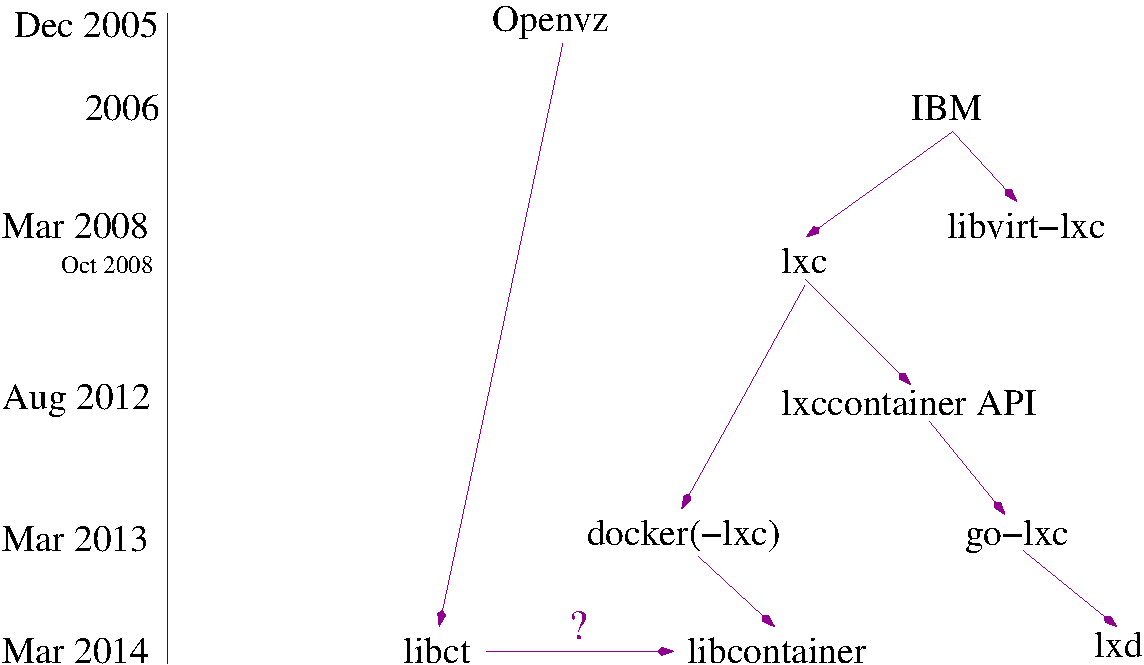
\includegraphics[width=\textwidth]{timeline.pdf}
\end{figure}
\end{frame}

\begin{frame}
\frametitle{Overview}
\begin{itemize}
\item 
\end{itemize}
\end{frame}

\begin{frame}
\frametitle{Openvz}
\begin{itemize}
\item Open sourced version of Virtuozzo
\item Full system containers
\item Very well liked
\item Required custom kernel patches
\item Being switched to libct
\end{itemize}
\end{frame}

\begin{frame}
\frametitle{Libvirt-lxc}
\begin{itemize}
\item Focus: Drive containers
\item Client-server
\item Non-root use of clients but not daemons
  \begin{itemize}
  \item Granting unpriv user == granting root
  \end{itemize}
\item Container creation through `virt-install'
\item Bindings
  \begin{itemize}
  \item C, python, Java, C\#, Perl, OCaml, Ruby, PHP
  \item Only for talking to daemon
  \end{itemize}
\end{itemize}
\end{frame}

\begin{frame}
\frametitle{Lxc}
\begin{itemize}
\item Focus: container management
\item API centered around own config language
\item Easy container creation from the start
\item Fully usable by non-root
\item Bindings
  \begin{itemize}
  \item C, python, lua, go, ruby, haskell
  \end{itemize}
\end{itemize}
\end{frame}

\begin{frame}
\frametitle{Libct}
\begin{itemize}
\item Focus: implement container drivers
\item Completely independent of
  \begin{itemize}
  \item config language
  \item container layout
  \end{itemize}
\item NO container creation
\item No support (yet) for non-root use
\item Support any combination of namespace sharing
\item Bindings
  \begin{itemize}
  \item C, python, go
  \end{itemize}
\end{itemize}
\end{frame}


%------------------------------------------------

\end{document} 
